\chapter{Background} \label{chapter:background}

\section{Existing Applications}

% overview

There are a number of existing applications available that attempt to solve the problem posed by this project. These range from fitness applications to various navigation applications, which although may not be completely relevant to this project, do provide some similar features such as place recognition that will be useful to research.

Table \ref{table:existing-walking-apps} shows how well each of the existing applications related to this project have implemented certain features. The maximum score for the feature category is displayed in brackets. The full matrix detailing what aspects each feature category is split into and why the score was given to each app can be seen in Appendix \ref{appendix:existing-apps-matrices}.

\begin{table}[htb]
  \centering
  \begin{tabular}{|m{2cm}||c|c|M{1.2cm}|M{1.5cm}|c|M{1.8cm}|}
    \hline
    \textbf{Features} & \textbf{MapMyWalk} & \textbf{Strava} & \textbf{Let's Walk} & \textbf{Google Maps} & \textbf{Citymapper} & \textbf{Pok\'{e}mon Go}\\
    \hline
    \hline
    Design (2) & 1 & 2 & 0 & 2 & 2 & 2\\
    \hline
    Ease of use (3) & 3 & 3 & 1 & 3 & 3 & 3\\
    \hline
    Tracking location (2) & 2 & 2 & 2 & 1 & 1 & 1\\
    \hline
    Navigation (4) & 3 & 1 & 1 & 3 & 1 & 2\\
    \hline
    Social interaction (5) & 2 & 2 & 2 & 0 & 0 & 0\\
    \hline
    \hline
    Total (16) & 11 & 10 & 6 & 8 & 7 & 9\\
    \hline
  \end{tabular}  
  \caption{Matrix showing how well existing walking apps perform at given features. Each app is given a score for a category, with the maximum score shown in brackets next to the feature category.}
  \label{table:existing-walking-apps}
\end{table}

The rest of this section discusses each application in detail, explaining their benefits and limitations. All of the applications researched are free to use unless stated otherwise.

% go through each existing app, discussing why they are good/bad with images

\subsection{MapMyWalk}

MapMyWalk \cite{Map} is a popular fitness application for iOS and Android that allows you to track your walks and complete challenges to help you keep fit. You are able to track a walk as you go on one, or log a previous workout that you have done without the app. The app also provides a premium subscription for \pounds4.49 per month, which gives you the ability to monitor your heart rate and set training goals that are designed to help you walk more.

The area in which MapMyWalk lacks is social interaction. A user can publish a walk that they have previously tracked to their profile, but there is no real aspect of communication with other users other than adding each other as friends. There is also a limited level of gamification in the app, with challenges being the only option available to encourage a higher rate of fitness. Challenges can either be added by the user or chosen from a precompiled list, with the latter being fairly limited in the range of options to choose from.

\subsection{Strava}

Strava \cite{StravaInc.} is another fitness application that primarily focuses on running and cycling. It features a sleek user interface with similar functionalities as MapMyWalk. The journey view within the application can switch between either showing the map of your workout or a statistics screen as shown in Figure \ref{fig:strava}, visibly showing the time elapsed in the workout, the distance travelled and your average pace per kilometre. Strava also provides a premium subscription for \pounds5.99 per month, which features personalised coaching and advanced analysis of your workouts.

The setback of Strava is that you cannot track walks in the app as you are constrained to either running or cycling. With regards to this project, it performs well in allowing the user to record and share their workouts but it does not provide any features for the user to explore areas around them. This is expected given that it is a fitness application and does not cater for walking whatsoever.

\begin{figure}[hbt]
  \centering
  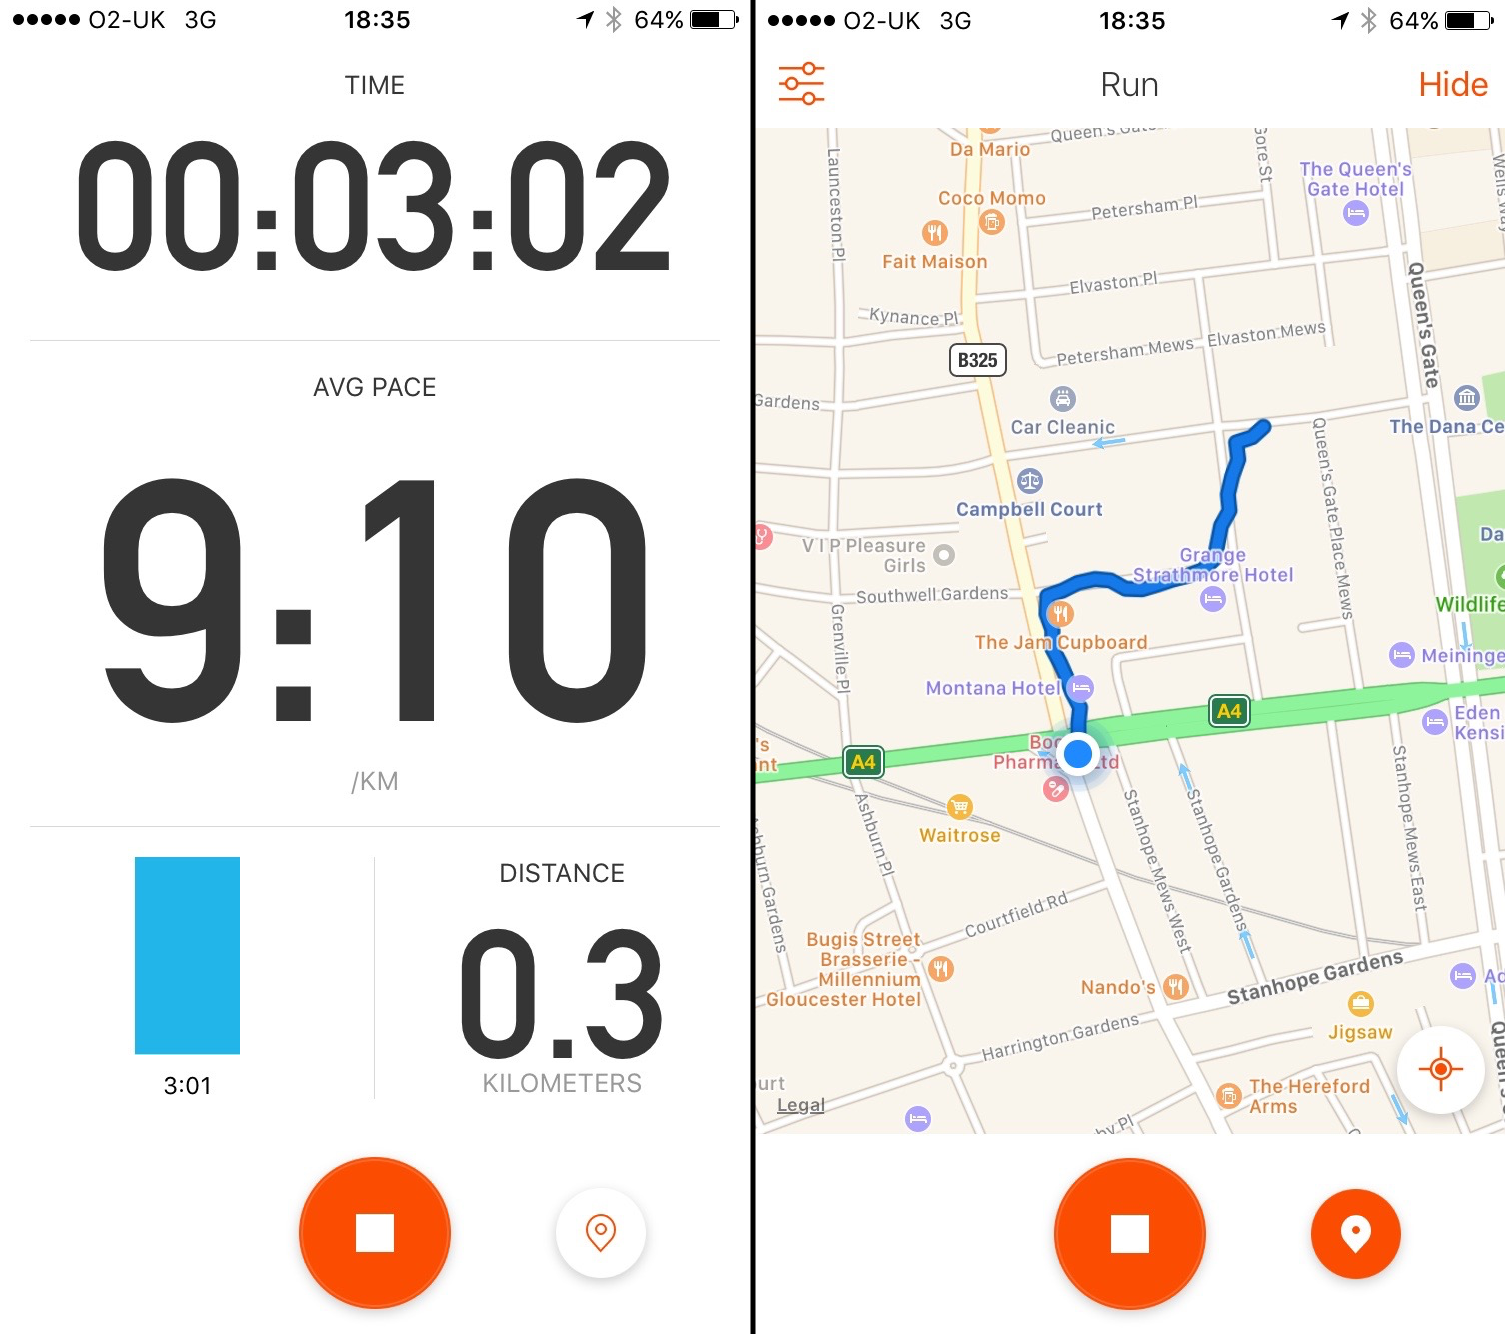
\includegraphics[width=0.7\textwidth]{strava}
  \caption{Journey view in Strava, allowing you to switch between statistics (left) or a map of your progress (right).}
  \label{fig:strava}
\end{figure}


\subsection{Let's Walk}

A lesser-known iOS fitness application is Let's Walk \cite{LetsWalkApp}. Users can record new walks and view a list of either their friends' walks or public walks nearby. The app is also focused on helping you maintain a balanced diet -- the amount of calories you consume can be added for particular meals during the day. A calorie goal per day can then be set, with the app recording how many calories were burned during a walk and updating the goal accordingly.

Let's Walk tries to emulate many of the features implemented by the more well-known apps as mentioned above, but a lot of these features seem unpolished. There is a global ranking section of the application showing which users have walked the most over the last week, month or year, however there seems to be little to do with this information other than view a leaderboard.



\subsection{Google Maps}

Although not a fitness application per say, Google Maps \cite{GoogleInc.} is one of the oldest services that provides route planning via different transport modes. The mobile app contains current information about public transport, traffic and displays well-known cycling routes on a map, however there is little in the way of customisation for walking. When entering a destination, the app generates a route but users can also choose from a few different routes on the map, with the app showing the difference in time each one would take. However, no information is given as to whether a certain route is quieter than another, for example.

\begin{figure}[hbt]
  \centering
  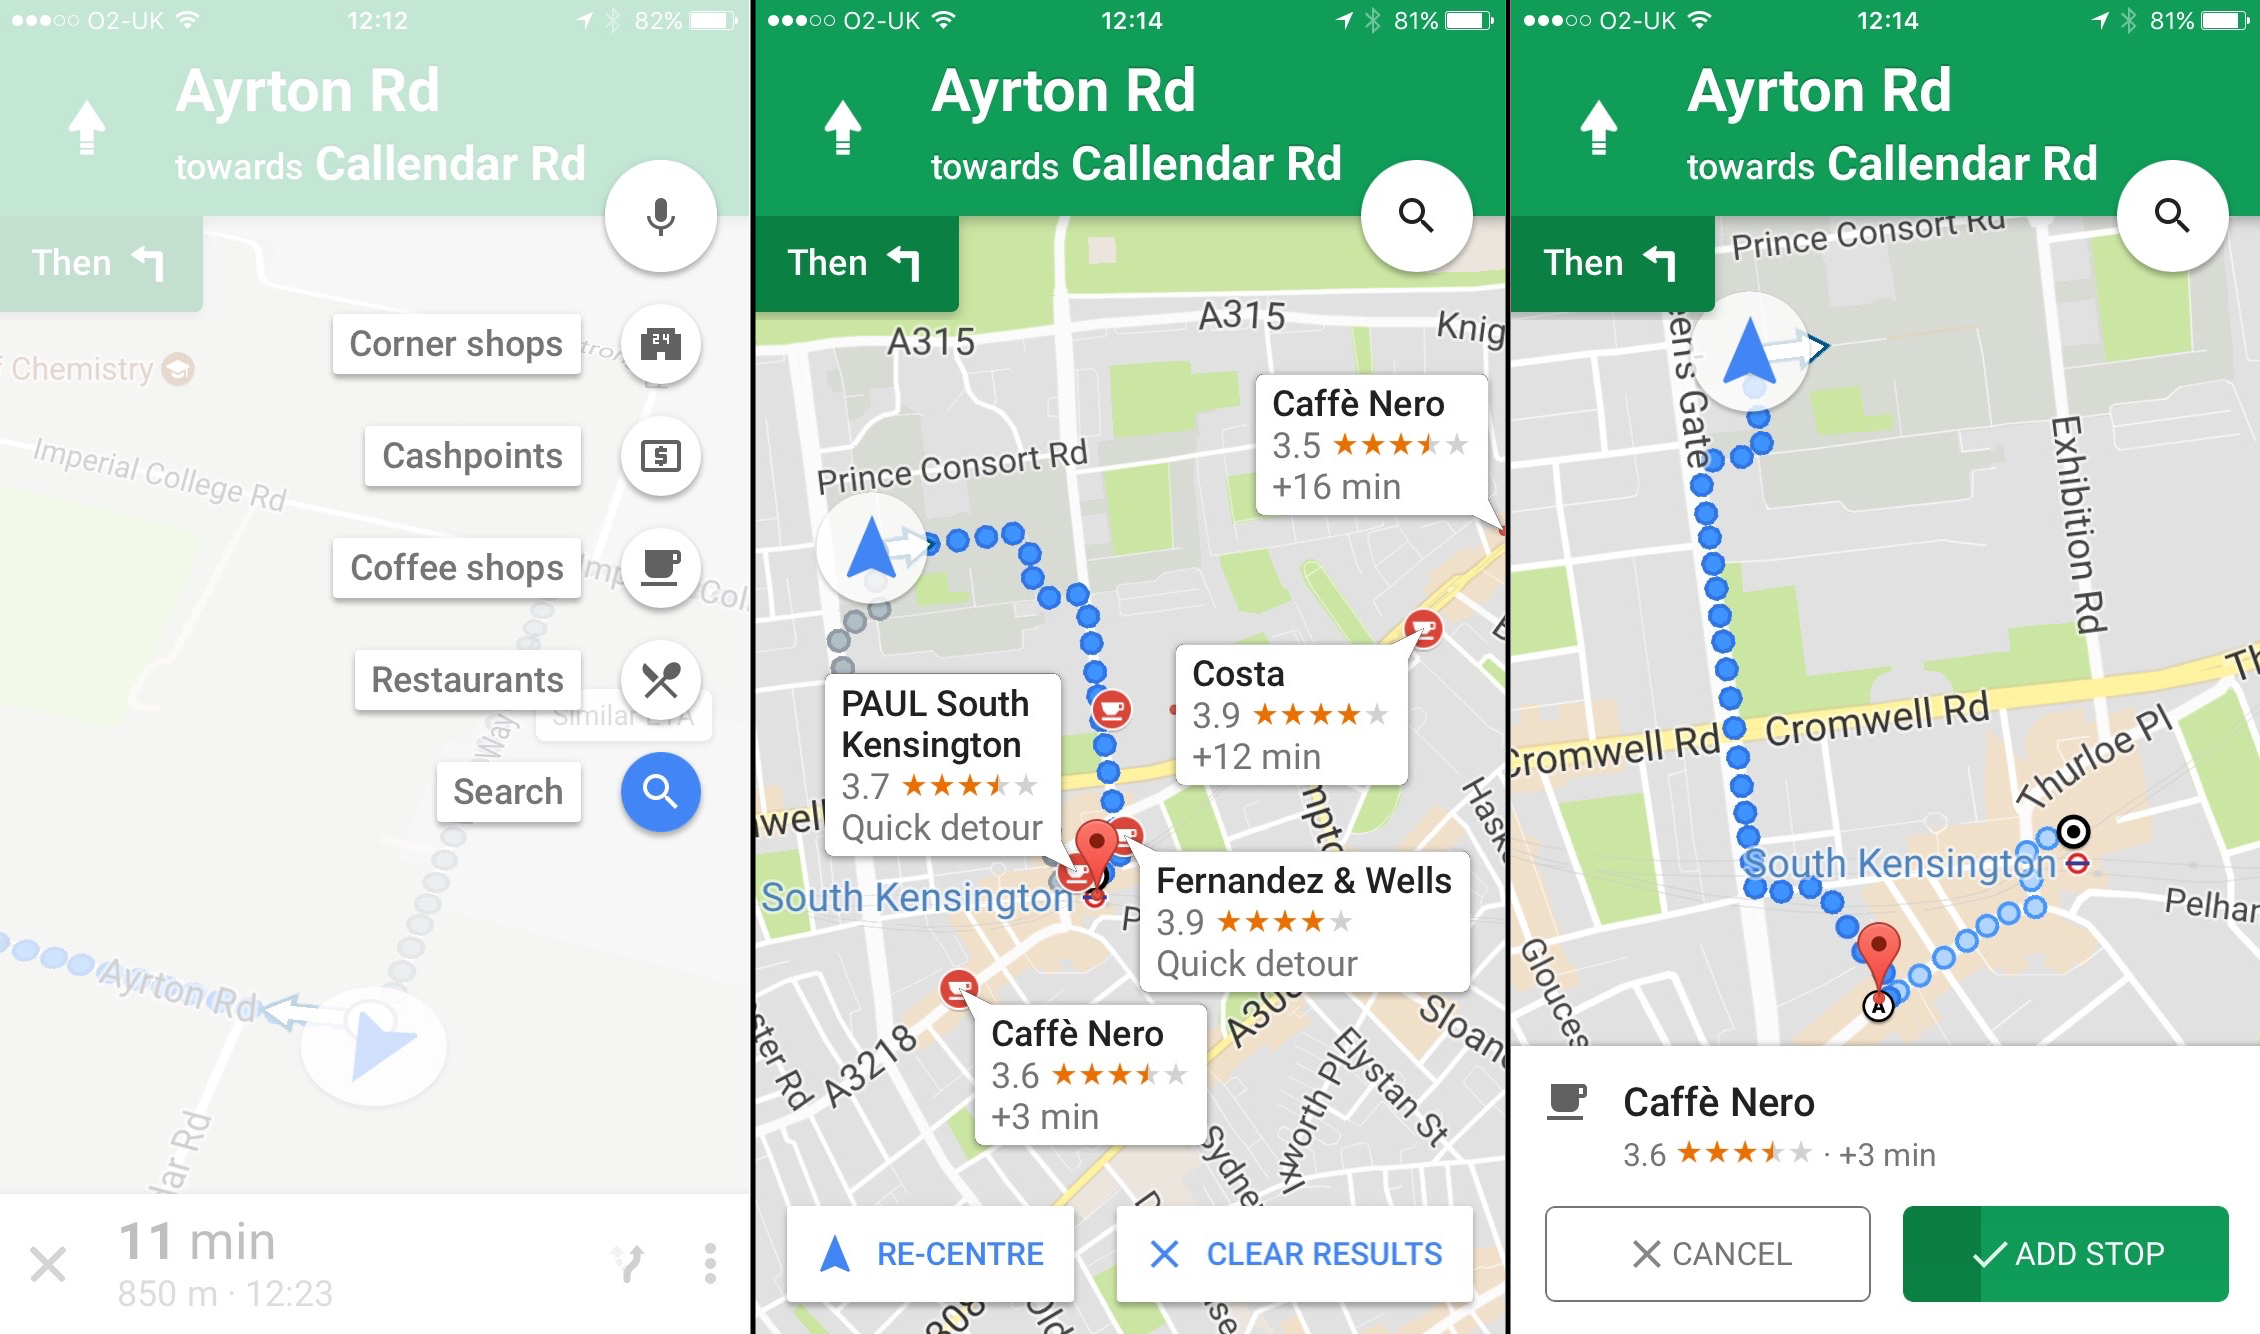
\includegraphics[width=\textwidth]{google_maps_place_search}
  \caption{Adding places along your walking route in Google Maps for iOS. A list of categories to choose from (left), then shows all the places from within a search on a map (middle). A stop can then be added and the journey will be updated (right).}
  \label{fig:google_maps_place_search}
\end{figure}


One feature of the Google Maps iOS application that is interesting to note is the ability to search for places along a route during a journey. Once a user has started a walking journey, they are able to search for places that are along the route. Google provides some categories of places to choose from, such as cashpoints and restaurants, but users can search for a specific place if they wish. The app will then display the results of the places search on the map, showing how much additional time would be added on to your journey if you were to stop at a place, if any. One or more places can then be added to your journey and the walking directions will subsequently update to include these new stops. Figure \ref{fig:google_maps_place_search} shows an example journey from Imperial College to South Kensington Underground station. It details the full process of choosing \textit{coffee shops} as the place category, selecting a particular coffee shop on the map and the stop being added to the journey.

The places search feature is important as it is unique within any of the existing journey planner apps I have researched and it relates to one of my objectives regarding displaying points of interest when a user is on a walk (\textbf{Obj 2}). More research is conducted in Section \ref{section:background-points-of-interest} to discover what tools these applications use to implement this feature.

\subsection{Citymapper}

Originating in London, Citymapper \cite{Citymapper} has become one of the leading journey planners for major cities around the world including Paris, Barcelona, New York, Tokyo and Sydney. One of the key features of Citymapper is that different modes of transport can be combined to create a faster journey time. For example, a journey from Imperial College to Oxford Circus (as shown in Figure \ref{fig:citymapper}) could just use the Tube, but it could be faster to hire a bike and cycle to a different station and then take the Tube.

\begin{figure}[hbt]
  \centering
  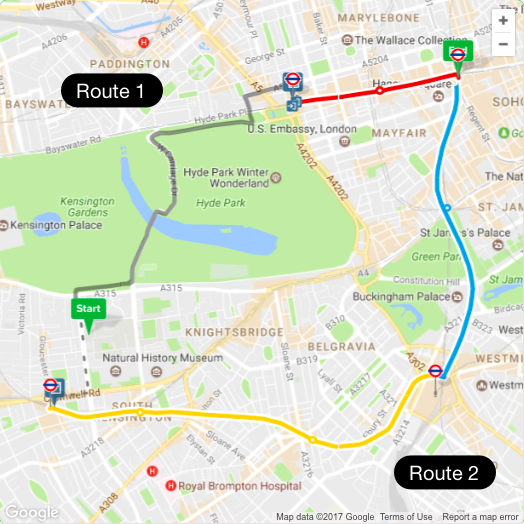
\includegraphics[width=0.7\textwidth]{citymapper}
  \caption{Two routes generated on the Citymapper website superimposed -- cycle and Tube route (Route 1) and Tube only route (Route 2).}
  \label{fig:citymapper}
\end{figure}

The walking directions in Citymapper are relatively limited. If you choose to walk on any route that you input, you are greeted with the screen shown in Figure \ref{fig:citymapper-walk}. Details such as estimated time of arrival, calorie burn and time of journey are displayed on this screen. Once you press \textit{Go}, you are transferred to the journey view, which simply tracks your location on a map and allows you to share your estimated time of arrival with others.

\begin{figure}[hbt]
  \centering
  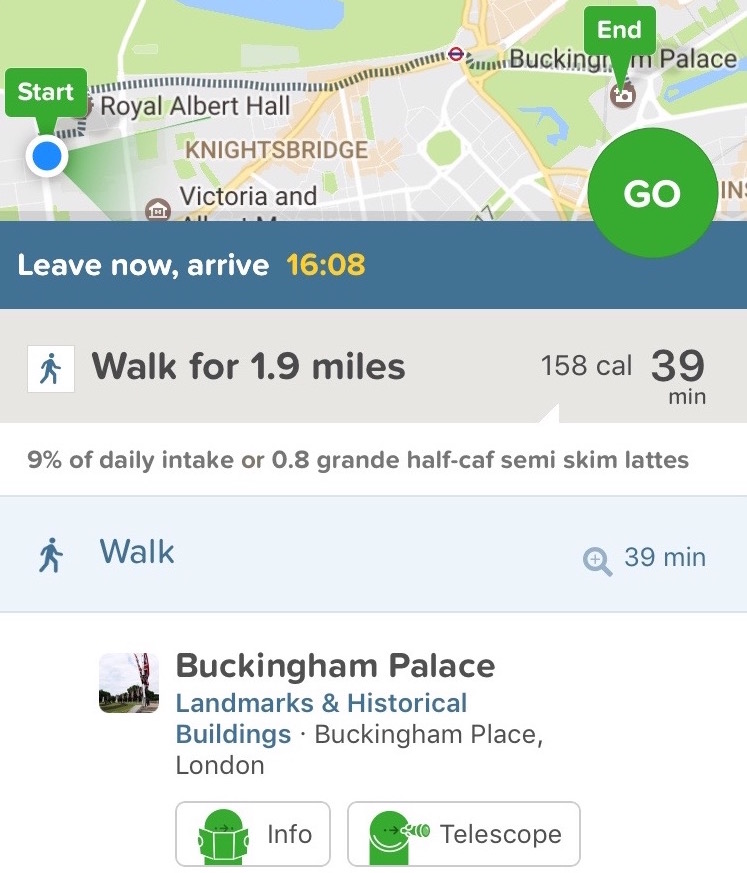
\includegraphics[width=0.55\textwidth]{citymapper_walk}
  \caption{Walking view in Citymapper}
  \label{fig:citymapper-walk}
\end{figure}

\subsection{Pok\'{e}mon Go} \label{subsection:pokemongo}

Pok\'{e}mon Go, released last July, quickly grew to become one of the most popular games of the year. Although not necessarily a walking application in the normal sense, the aim of the game is to capture virtual `creatures' called Pok\'{e}mon that appear in real world places. Thus, the game motivates you to walk more to collect more and more Pok\'{e}mon.

One of the more interesting parts of the application that is relevant to this project are the Pok\'{e}stops within the game. A Pok\'{e}stop is a location in the game where various in-game items can be collected. They are displayed on a map using blue beacons as shown in Figure \ref{fig:pokemongo}. These locations were crowdsourced by users of the game and are normally points of interest in the area such as a statue, a building or a famous plaque. Although not completely, this feature of the application does somewhat tie into my objective for helping people discover the world (\textbf{Obj 2}).

\begin{figure}[hbt]
  \centering
  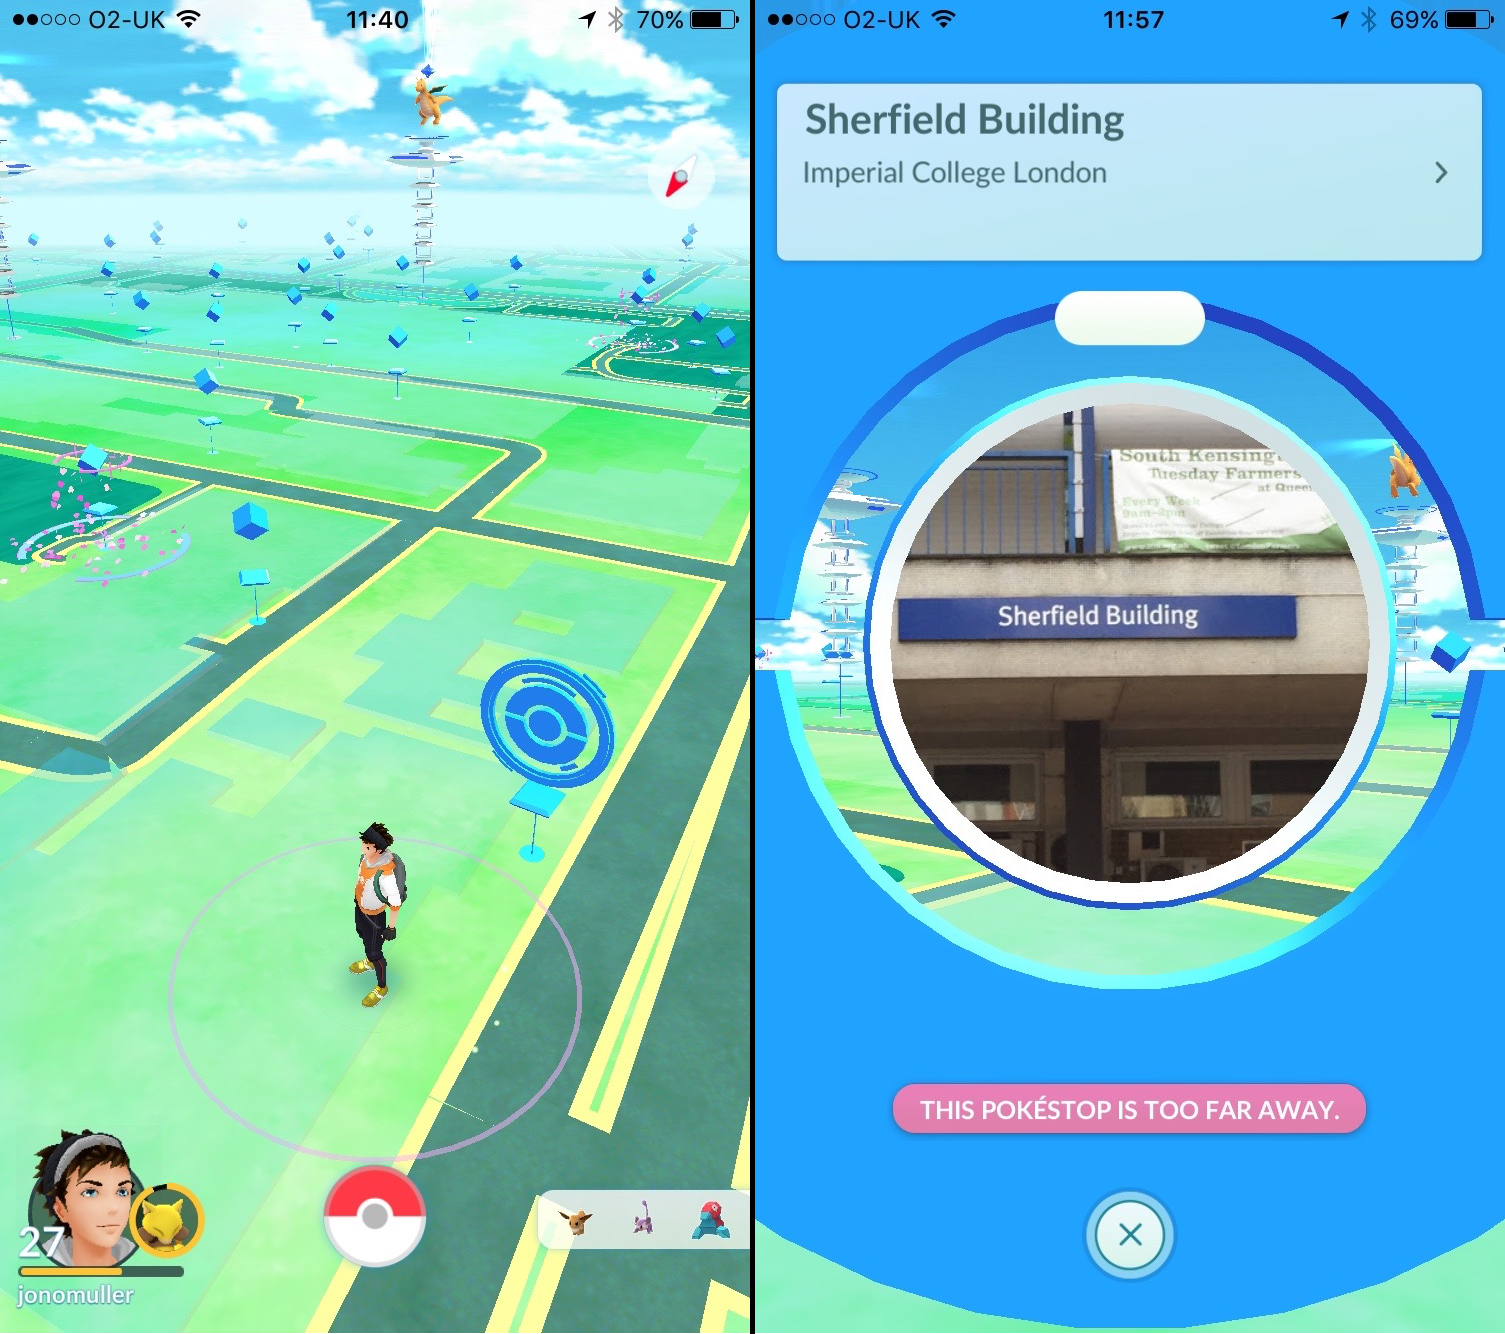
\includegraphics[width=0.7\textwidth]{pokemongo}
  \caption{Screenshots of Pok\'{e}mon Go showing Pok\'{e}stops in an area (left) and a detailed view of a Pok\'{e}stop (right).}
  \label{fig:pokemongo}
\end{figure}

\subsection{Summary}

From the subset of fitness applications that I researched in this section, it can be seen that some of the objectives I proposed in Section \ref{section:objectives} have been achieved but no single application encompasses all of my proposed objectives. I have found that it is important for this project to have a sleek design and easy-to-use interface as this is something that stood out straight away when looking at existing applications.

%\pagebreak

\section{Gamification}

% research how gamification has been used in applications, not just walking apps
% discuss how well each implementation has worked

Gamification is used in mobile applications not only for fitness but also in a wide range of areas including productivity, finance and mental health. We have seen how gamification can be used in existing fitness applications, with some apps setting challenges for users to complete within a given timeframe -- such as running a half marathon in February.

This section discusses the alternative uses of gamification in existing applications, followed by the way in which gamification could be used in this project.

\subsection{Alternative Uses}

An application and website called Habitica \cite{Habitica}, labelled as a ``gamified task manager", helps motivate you to complete household tasks by unlocking features and levelling up an in-game avatar. Completing real-life tasks earns you gold for your character, which can then be redeemed for either virtual rewards such as equipment or real-life treats like watching an episode of a TV show, for example. The home page of Habitica, shown in Figure \ref{fig:habitica}, is split into columns containing your bad habits, daily tasks, to-do list and rewards. It also shows the progress of your avatar, along with what is needed to progress to the next level. This type of app helps you become more productive at home in a fun and creative way that users enjoy.

\begin{figure}[hbt]
  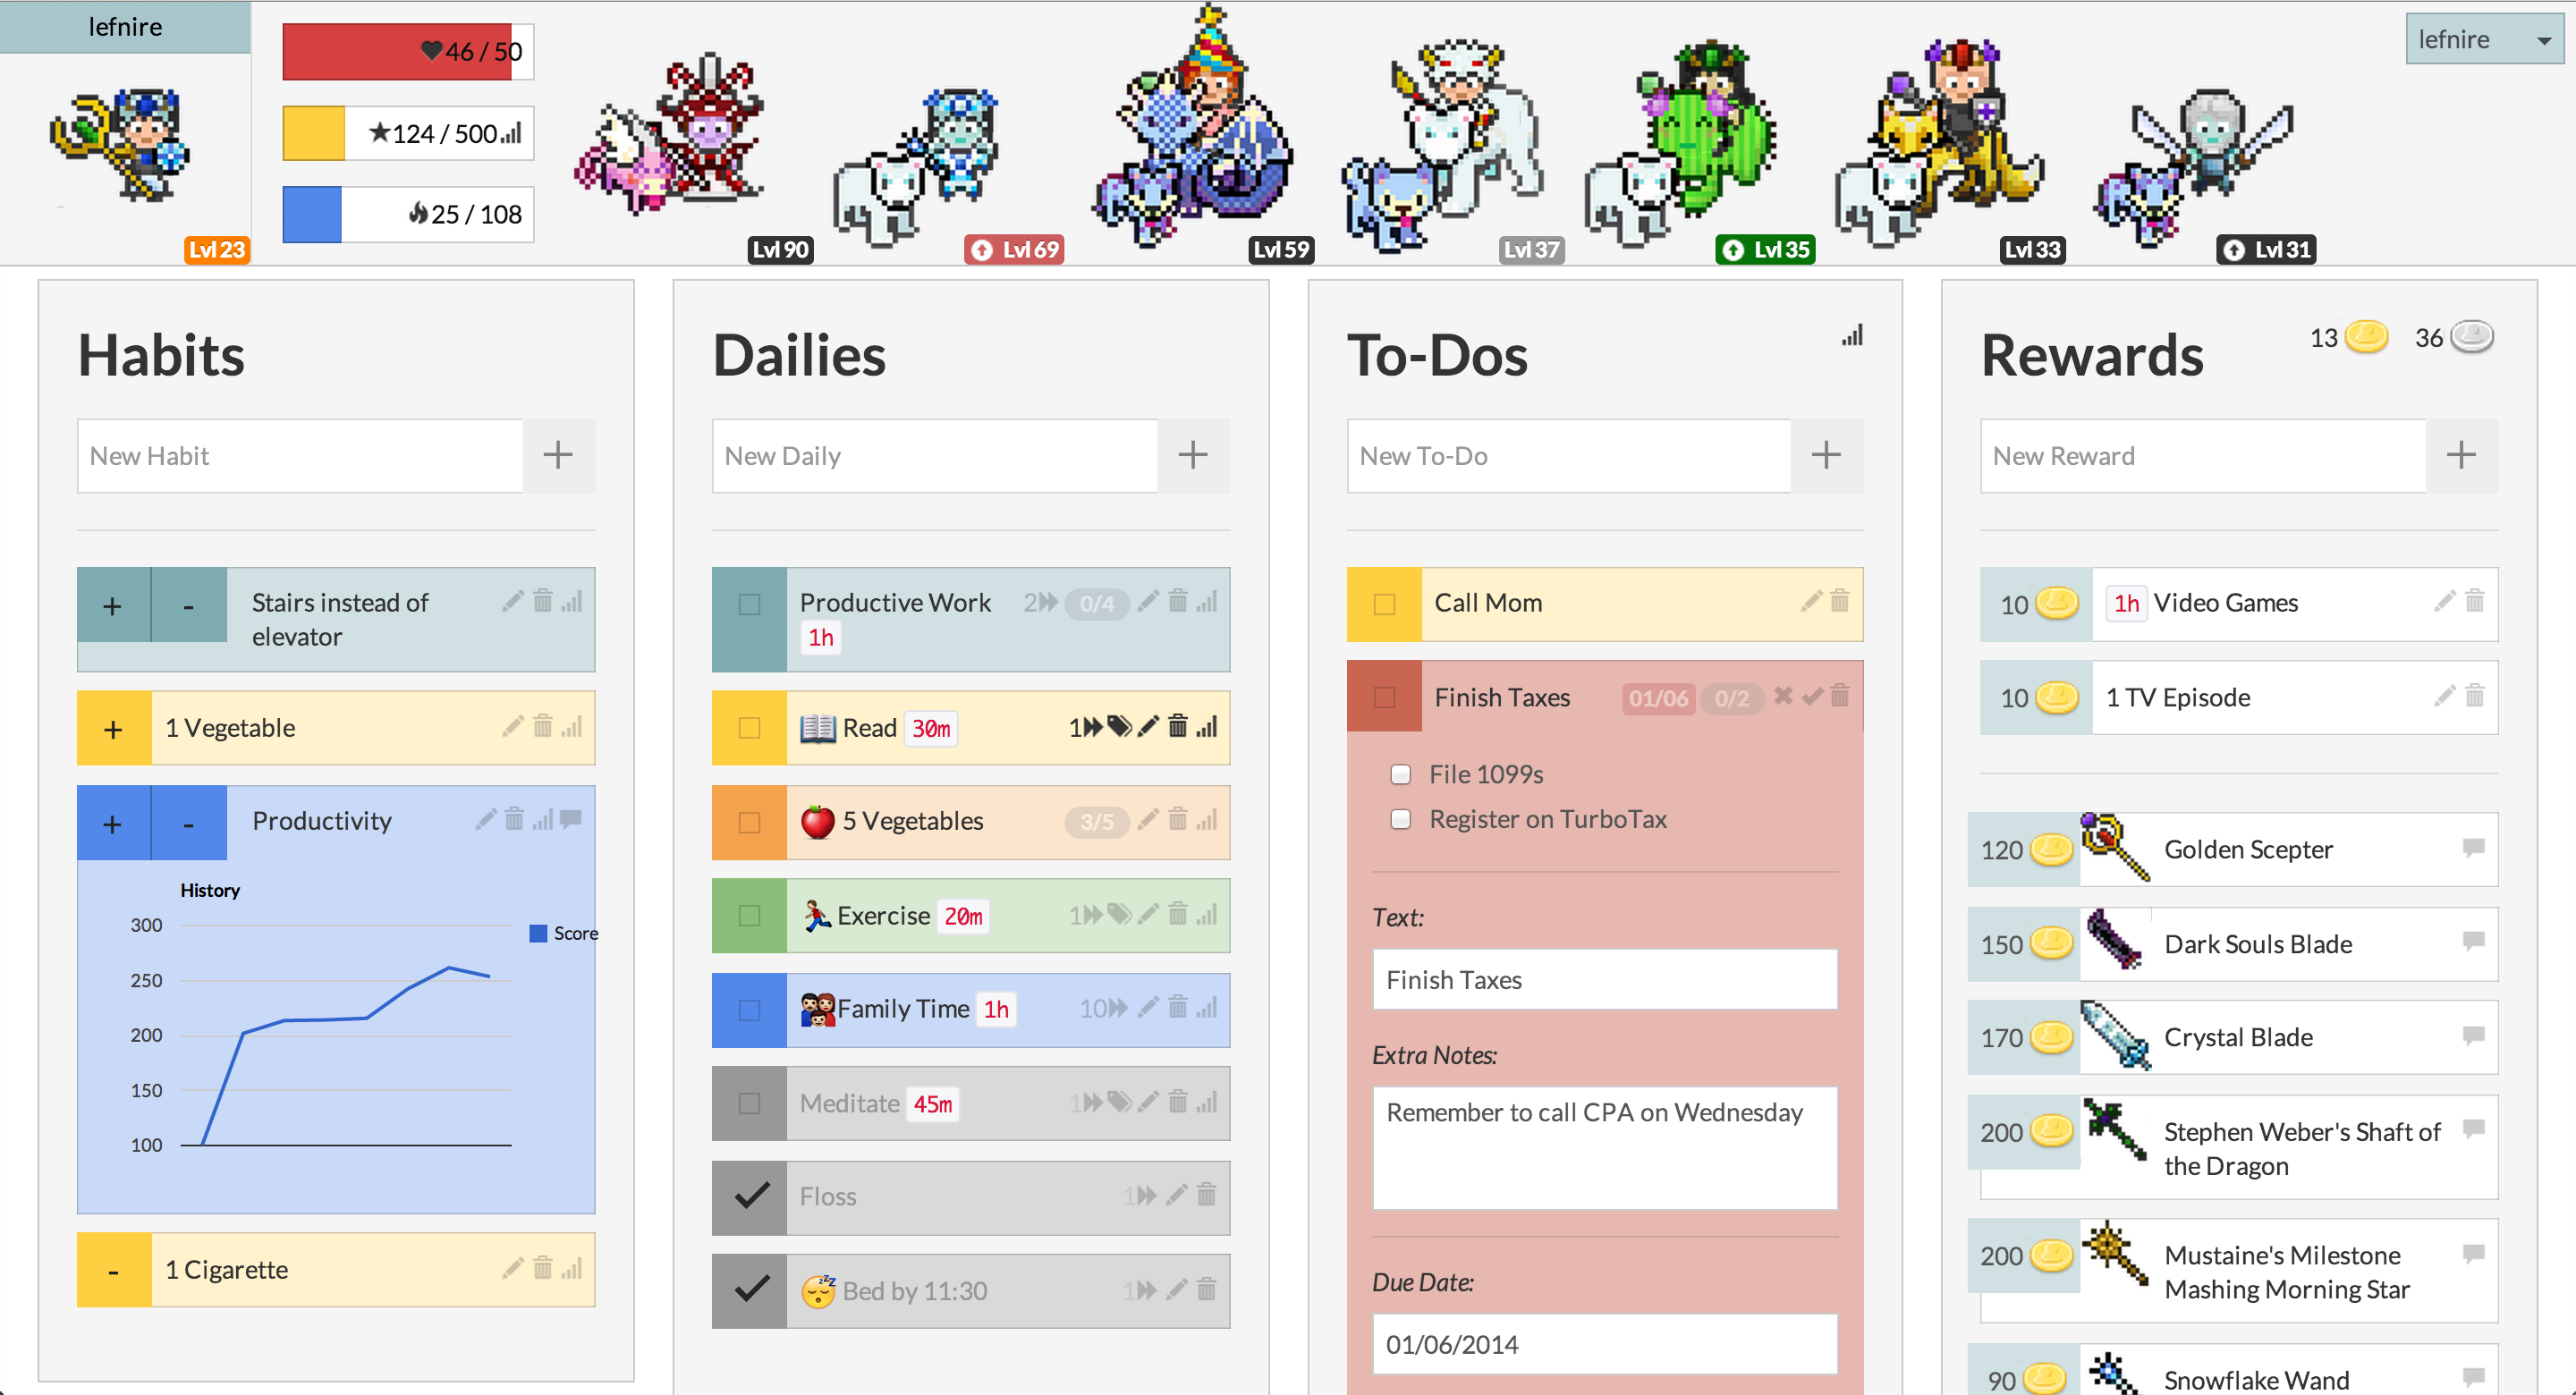
\includegraphics[width=\textwidth]{habitica}
  \caption{Home page of Habitica showing your habits, tasks and rewards as well as your avatar at the top \cite{Habiticaa}}
  \label{fig:habitica}
\end{figure}

Gamification is also used in some finance applications. Mint \cite{IntuitInc.} is an application available in America that links to your bank accounts to help you manage your bills and track how much money you spend. It shows a breakdown of what you are spending your money on and creates a budget with the option of using any left over money on goals designed to help you save money, as shown in Figure \ref{fig:mint}. You can create goals to be either a long-term one-off payment -- buying a house, for example -- or a short-term monthly payment such as a subscription service. This game mechanic of working towards a goal to help you buy something you want is extremely effective and is why gamification is so widespread.

\begin{figure}[hbt]
  \centering
  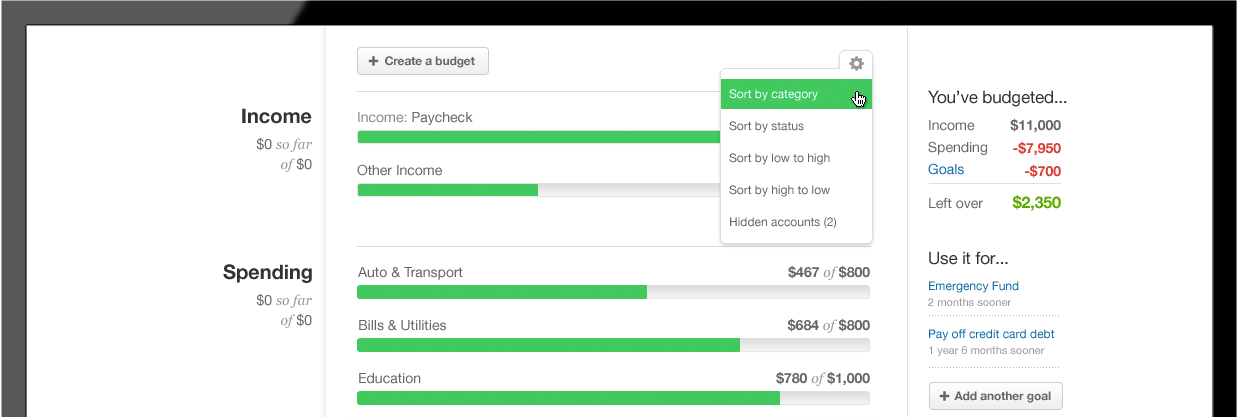
\includegraphics[width=\textwidth]{mint}
  \caption{The breakdown of spending in Mint, giving you the option to use any left over money from your budget for one or more goals \cite{IntuitInc.a}}
  \label{fig:mint}
\end{figure}

The idea of using gamification in applications is to motivate you to complete some form of task that you otherwise might not have attempted. It can make an app seem more engaging to the user, providing them with something to achieve every time they use the app. It is especially useful in fitness applications as keeping fit and staying healthy is very important, and should therefore be carefully considered for this project.

\subsection{Summary} \label{subsection:background-gamification-summary}

In terms of this project, I had to consider two main factors regarding the type of gamification to use: its usefulness to the user and the feasibility of implementation. I discussed with potential users the extent to which they thought gamification should be used, ranging from a achievements-based system to a full character game. While some did say that the game aspect would be fun, many said the way that would motivate them to exercise more would be an achievements and scoring system. Achievements (and points) would be gained the more you walk, with the points contributing to a tally on the user's profile.

From this, I created a list of achievements that I found would be most useful to implement initially.

\begin{itemize}
  \item \textbf{Distance:} earned for every walk. The further you walk, the higher number of points will be gained.
  \item \textbf{Streak:} earned if you walk everyday for a number of days, forming a walking streak. The number of points gained is based on how many days are in the streak.
  \item \textbf{Group exercise:} earned if you walk in a group, with the number of points depending on how many people there are.
\end{itemize}

The use of achievements also allows for extensibility in the future, with more able to be added at any time.

\section{Points of Interest} \label{section:background-points-of-interest}

In order to achieve my proposed objective of helping users discover more of the world around them (\textbf{Obj 2}), I had to research which sources would be able to provide me with nearby points of interest based on a location.

\subsection{Google Places API}

Google's Places API \cite{GoogleInc.b} would be a good resource to use, allowing you to search for places by over a hundred types including \textit{point of interest}, \textit{place of worship} and \textit{museum}. One issue with using Google Places is that you must use Google Maps to display the places on. From the Google Places Policies, \textit{``If your application displays data from the Google Places API for iOS on a map, that map must be a Google map"} \cite{GoogleInc.c}. I would need to consider this issue when choosing the map source to use for the application, which is discussed in Section \ref{subsection:background-apis}.

\subsection{MKLocalSearch}

Apple provides a framework for obtaining places called \texttt{MKLocalSearch} \cite{AppleInc.b}. To generate a list of places, you pass the \texttt{init()} method a \texttt{MKLocalSearchRequest}, which contains a `natural language query` string describing what type of place you would like to search for on a map.

There seems to be little documentation online explaining what range of places this API returns. After some initial testing, I found that the downside of this service is the natural language search query -- you cannot search by the type of place. This results in unintended results being returned from a request. As an example, to find any monuments nearby you would search for the keyword \textit{monument}, but the search results will include Monument Underground station.

% talk about no types,
% monument could return monument station -> not intended

\subsection{Pok\'{e}stops}

A different option that could be used to generate points of interest around a geographical location originates from Pok\'{e}mon Go. As mentioned in Section \ref{subsection:pokemongo}, Pok\'{e}mon Go contains thousands of Pok\'{e}stops -- crowdsourced points of interest from all over the world. There exists an API \cite{Selwyn} that returns a list of Pok\'{e}stops in JSON format given a location. Each item that the API returns contains the name and location of a point of interest, as shown in Listing \ref{listing:pokestop}, and so could therefore be used in this project.

\medskip

\begin{listing}
  \centering
  \begin{lstlisting}[style=json]
  {
      "distance": 44, 
      "name": "Sherfield Building", 
      "bearing": 200, 
      "latitude": 51.498359, 
      "image": "http://lh3.googleusercontent.com/07q4ms3tgDKsQMy04xye
            <@\textcolor{red}{\hspace*{20pt}\_i-UiraPO3jOS18TXwKpTMecgIXm2jXByO1CAUWVW9vNgqfx12ZtjqLdZrOlfsPu}@>", 
      "guid": "2cc0f9d9c7ba49348299c15749c49ea1.16", 
      "compass": "S", 
      "longitude": -0.178544
  }, 
  \end{lstlisting}
  \caption{Example of one item returned from the Pok\'{e}stop API, with attributes including its name, latitude, longitude and distance from your location}
  \label{listing:pokestop}
\end{listing}

\subsection{Historical Plaques}

Based on initial feedback of the project, users suggested that the multitude of `blue plaques' around London would be a good way to display points of interest. These plaques are placed on buildings and public places in London to commemorate a notable person or place in history. The blue plaque scheme is administered by English Heritage \cite{EnglishHeritageTrust}, a charitable organisation responsible for the upkeep of over 400 historical sites across the United Kingdom.

All data from the plaques from English Heritage is publicly available by request under the Freedom of Information Act 2000 -- an act to publicise information held by public institutions. The English Heritage website provides an option to search for a plaque given a query string, however there does not seem to be an option to search for plaques given a map area, meaning it would not be that effective for the purposes of this project. A request to retrieve all plaque data from English Heritage would both be tedious and a waste of space, so I therefore needed to look for another option.

I came upon an open source service in OpenPlaques \cite{OpenPlaques} -- a collection of plaques run by volunteers, which seemed to be well populated. OpenPlaques contains all the English Heritage blue plaques from London, but also other plaques around the UK and the world that various other organisations have put up. OpenPlaques also offers an API that supports querying plaques in an area by supplying a bounding box.

\subsection{Summary}

The options discussed all provide extremely different ways to retrieve points of interest. Both Google's and Apple's services may be the most convenient -- as they would be integrated into the map source chosen -- but they both contain limitations, most importantly that there is no extra information returned about a point of interest other than its title.

The other two services that use Pok\'{e}stops and historical plaques provide, in my opinion, a more appealing approach to finding new points of interest in an area. Based on my own thoughts and the thoughts of users I asked, I chose to use the latter option as the source of points of interest for the project. Using historical plaques seemed the more interesting option to enable the user to learn about places and motivate them to investigate more into these places, which is essentially what my aim was.

% not sure whether to include this in background or design?
% think I will include general background on technologies here, and then which ones I chose in design
\section{Technologies} \label{section:technologies}

The features of existing applications are not the only important part to research -- the technologies that they use to implement these features are just as useful. This section discusses how existing applications implement certain features and which technologies integrate well with each other.

\subsection{Mobile Operating System}

Many of the applications that I have researched have been developed for iOS, the operating system running on iPhones and iPads. I have chosen to develop my application on iOS due to my previous experience with iOS app development. Another factor in this choice is that I have gained a lot of experience programming in Swift, one of the programming languages used to develop iOS apps, over the last few years. Swift is extremely readable and easy to use, which is the reason why I am choosing to use it over the other programming language available, Objective-C. I am also familiar with the tools required to develop an iOS application, specifically the integrated development environment (IDE) Xcode.

\subsection{Version Control} \label{subsection:version-control}

Version control is a crucial part of the development process with any project, especially this implementation-heavy project. It provides a full history of changes made to a codebase along with the ability to revert back to previous versions of code and work simultaneously on different features by creating branches. Git and GitHub are my chosen version control system and platform respectively due to past experience and familiarity.

Along with version control, errors or bugs in code must be detected quickly in order to not hinder the development process. To do this, the practice of continuous integration (CI) was used to integrate and test code frequently, making it easier to locate the origin of an error. There are many CI tools that can be used to automate code testing including Jenkins, Travis CI and BuddyBuild. I had no prior knowledge with any of these tools and so I researched the benefits and drawbacks of each service, which can be seen in Table \ref{table:ci-tools-options}.

\begin{table}[hbt]
  \centering
  \begin{tabular}{|m{1.5cm}||M{3cm}|M{3cm}|M{3cm}|M{3cm}|}
    \hline
     & \textbf{Jenkins} & \textbf{Travis CI} & \textbf{BuddyBuild} & \textbf{GitLab CI} \\
    \hline
    \hline
    Platform & Windows, macOS, Linux & Hosted & Hosted & Hosted on GitLab\\
    \hline
    Cost & Free & Free for students & $\sim$\pounds55/month or free trial & Free for small individual projects\\
    \hline
    Main Feature & Plugins available for variety of languages & Linked well with GitHub & Designed solely for mobile development & Integrated with GitLab\\
    \hline
    Platform Specific & No & No & Yes & No\\
    \hline
  \end{tabular}
  \caption{Comparison of continuous integration tools}
  \label{table:ci-tools-options}
\end{table}

I concluded that Travis CI was the most suitable option for me since it was hosted on GitHub and is not platform specific, meaning that I could use it to test both the mobile app and API even though they were written in different languages. Using an option like BuddyBuild could only be used for the mobile app, with another tool needed for the API.

\subsection{Location Tracking}

To track the user's location within iOS, an application can use the classes from the Core Location framework \cite{AppleInc.} inbuilt into the iOS SDK (software development kit). This framework allows a developer to obtain the user's current location in the form of latitude and longitude. To keep a history of where the user has been, these coordinates could be stored in an array and updated every few seconds. This will be useful for my application to show on a map where a user has previously walked.

% section on how to track calories burned?

\subsection{Map Source} \label{subsection:background-apis}

One of the most important technology aspects to consider is which source of map to use. The majority of existing applications use Apple's maps apart from, of course, Google Maps. This is because Apple's MapKit framework \cite{AppleInc.a} is much better integrated with the Core Location framework mentioned above, making it much easier to display the user's location on MapKit than on the Google Maps SDK. It also provides convenient functions for coordinate conversions and calculating distances between two coordinates, which is useful for this project when trying to calculate the distance of a tracked walk.

% maybe don't include
However, there are some advantages of Google Maps over Apple Maps -- one being that Google Maps tends to be more detailed than Apple Maps. An example of this is shown in Figure \ref{fig:google-apple}, where in my opinion roads are easier to see and buildings are clearly visible on Google Maps than on Apple Maps.

\begin{figure}[hbt]
  \centering
  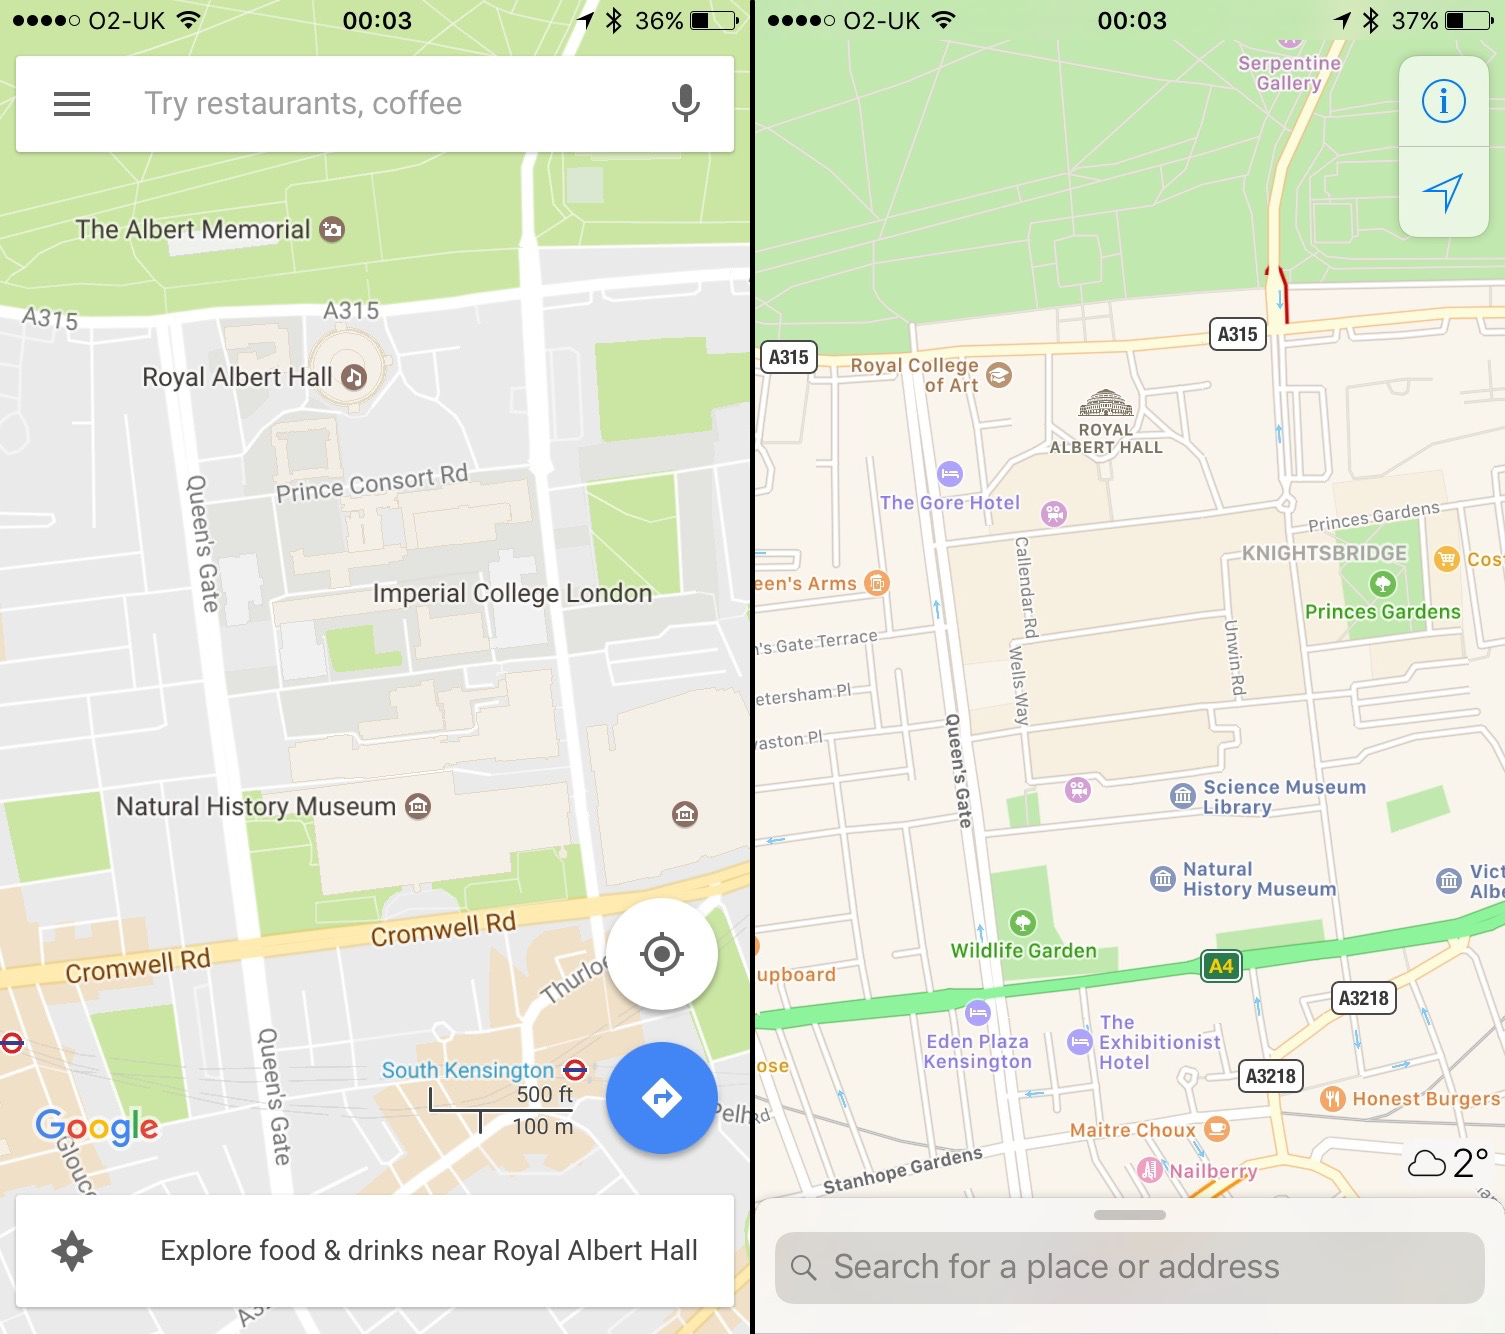
\includegraphics[width=0.7\textwidth]{google-apple}
  \caption{An example of the difference between Google Maps (left) and Apple Maps (right), showing Imperial College London.}
  \label{fig:google-apple}
\end{figure}

%As discussed in Section \ref{subsection:background-apis}, Apple Maps very well integrated with the Core Location framework in iOS, which makes it easier to deal with displaying the user's location on a map. 

For the reasons listed above, I chose to use Apple Maps and their MapKit framework as the source of maps within the application. The one issue of the lack of detail in some areas of the maps was not deemed important enough to impact my decision and did not outweigh the benefits of the MapKit framework that are listed above.







% add section on blue plaque API
% used based on data from research survey





%\section{Technology Choices}

%The first part of the design of the project is to consider which technologies to use. The technologies that I chose stemmed either from the background research I conducted in the previous section or previous personal knowledge.

%\subsection{Mobile Operating System}

% move section in background to here?


% *** points of interest APIs ***

\subsection{Server Architecture} \label{subsection:server-architecture}

Before deciding what specific technologies to choose for the server, such as the programming language, we must consider the type of architectural style to use. The aim of the API exposed by the server is to provide an abstraction between complex database queries and provide functionality that a client can use to query and update details. The Representational state transfer (REST) architectural principle fit the needs for this aim very well. Every component in a RESTful web service is a resource that can be accessed via the standard HTTP methods, including \textit{GET}, \textit{POST} and \textit{DELETE}. In comparison with other web services, such as the Simple Object Access Protocol (SOAP), RESTful services have much less overhead when sending data due to the extra XML header information sent when using SOAP.

With the architecture chosen, I assessed the options for the language to write the API in. There are a wide range of programming languages that could be used, and it came down to personal preference and how well it would suit the needs for this project. The popular options include PHP, Ruby, Python and Node.js \cite{Node.jsFoundation} -- the server-side environment run in Javascript. The only language in this list that I have experience in is Python, which would mean I would have to spend less time learning the language if I were to choose it. However, the advantage of Node.js for the purpose of this project is that objects in Javascript are built using Javascript Object Notation (JSON).

 RESTful web services support the use of multiple different data formats to serialise responses from the server, including HTML, XML and JSON. By choosing Node.js as the server language and JSON as the data type, I was able to easily parse data from HTTP requests and send responses in JSON, despite not having any previous experience with Javascript.

\subsection{Database}

There are two types of database that could be used: relational or non-relational. Relational databases are based upon relational algebra where data is stored in tables with queries to this data in the form of Structured Query Language (SQL). Each table in a relational database normally identifies a type of entity, and each instance of that entity is uniquely identifiable so that it can be referenced in other tables. SQL therefore supports the querying of this data across multiple tables using relational operators such as joining two tables. The most used services to model data in a relational database are MySQL and PostgreSQL, with the latter providing support for storing arrays -- a useful feature for this project as the coordinates of a walk need to be stored.

The opposite of this data model is a non-relational, or NoSQL, database in which each data entry is stored as a JSON-like document. This approach has many advantages for this project, primarily the similar use of JSON to both store data and build objects from in Node.js. As a result, data can be queried or inserted directly from a network request without any type conversions. NoSQL databases also have the benefit of faster query speeds and the ability to scale data horizontally -- an important factor to consider when designing a database.

The leading service to use for managing document-based NoSQL databases is MongoDB. It was used in this project especially due to its similar use of Javascript and JSON, both of which are already employed in the Node.js API. I also used a popular object data modelling library, Mongoose \cite{Mongoose}, which helped with validation and allowed me to define schemas for each of the type entities.

\subsection{API Deployment}

I opted to host my API on the platform-as-a-service Heroku \cite{Heroku2016}, with the alternative being Imperial's Cloudstack service run by the Department of Computing. Having had little experience with either of these services, I learned that Heroku had certain features that gained itself an advantage over Cloudstack.

Heroku is integrated with GitHub very well, my chosen version control platform, supporting automatic deployment when commits are made that can also be dependent on the results of continuous integration tests. Heroku also has a number of add-ons that can be used on web applications, including mLab -- a cloud-hosted version of MongoDB that is essential for me following on from the choice of database discussed in the previous section. Conversely, Cloudstack does not support MongoDB outright and would therefore take more time to set it up.

\subsection{File Storage}

An online file storage system was needed for the project to store thumbnail images of tracked walks, which is discussed in more detail in Section \ref{subsection:file-storage-methods}. Due to the ephemeral nature of Heroku's file system, it is not possible to store permanent files there and therefore an alternative online file storage service must be used.

From the wide range of services available, there is one stand-out option that I chose to use -- Amazon's simple storage service known as AWS S3. Its free usage tier allows up to 5GB of data storage which would be plenty for the purposes of this project. It also provides an SDK for Javascript which was necessary in order to implement the storing and deletion of images from the API.

\section{Summary}

The outcome of the background research of the project has enabled me to narrow down the requirements that I want to complete. Researching existing fitness applications was useful to determine the way in which workouts are recorded, as well as the range of ways gamification is used. Alternative uses of gamification provided a different approach, including gaining rewards for completing household chores, however I chose to use an achievements-based system based on user feedback. The result of the points of interest research is a service that provides interest and motivation for the user -- a core objective of the project.

Finally, I was able to choose the technologies that would suit the project best based on the conclusion of the previous research. We can now create a detailed list of requirements that should be completed in the project, and begin to design and implement these requirements.






